\chapter{Algoritmo Genético}

\section{Introducción}

\subsection{$r_v = ICESym(motor)$}
%
ICESym lee un archivo de configuración en formato \emph{Python} que consta de
un arrego llamado \emph{diccionario} con las siguientes entradas:

\begin{lstlisting}[language=Python]
kargs = {
    "Simulator": Simulator,
    "Cylinders": Cylinders,
    "Junctions": Junctions,
    "Tubes": Tubes,
    "Tanks": Tanks,
    "Atmospheres": Atmospheres,
}
\end{lstlisting}

En donde se guarda la información básica de la geometría del motor, modelos
termodinámicos utilizados, cantidad de RPM's a simuilar y modelo de Cd entre
otros.

% De manera resumda, son básicamente métodos de búsqueda aleatoria que
% aprovechan la información de iteraciones previas para determinar la composición
% futura de la población, representando individuos como un conjunto de datos.
% La representación
% %
% Si bien es probable que no se alcance el óptimo, el método alcanza una solución
% satisfactoria en un tiempo relativamente corto.


% Los AG requieren que las variables del problema estén expresadas en forma de
% coordenadas $(x_1, x_2, x_3, ..., x_n)$.





\section{Componentes básicos}
%



\section{Implementación}

\subsection{Población}
%
Los parámetros que representan a cada individuo son los que definen la geometría
del sistema de intercambio de gases, estos son:

\begin{enumerate}
    \item [DTA] Diámetro de tubo de admisión.
    \item [DTE] Diámetro de tubo de escape.
    \item [LIT] Largo de tubo de admisión.
    \item [LET] Largo de tubo de escape.
    \item [IIA] Ángulo geométrico de apertura de puerto de admisión.
    \item [IFA] Ángulo geométrico de cierre de puerto de admisión.
    \item [IIE] Ángulo geométrico de apertura de puerto de escape.
    \item [IFE] Ángulo geométrico de cierre de puerto de escape.
\end{enumerate}

Los diámetros pueden tomar valores de hasta 100mm, el largo de los tubos puede
variar entre 500 y 1000 mm.
%
Con respecto al par de ángulos que marcan la apertura y cierre del ecape,
el único requisito es que la apertura se de antes que el escape.

\begin{lstlisting}[language=Python]
def check_angles(eng):
    """ Validates intake/exhaust angle pair"""
    iia = eng[-4]
    ifa = eng[-3]
    eia = eng[-2]
    efa = eng[-1]
    valid = True
    if iia >= ifa:
        valid = False
    if eia <= efa:
        valid = False
    return valid
\end{lstlisting}

Cada una de las variables se representa como un número binario de 5 dígitos,
los cuales se concatenan para formar un conjunto de 40 dígitos.
%
Estos 8 números binarios se convierten mediante una transformación lineal
al número que se envía a ICESym.

\begin{table}
    \centering
        \begin{tabular}{rc} \toprule
            No. & String                                   \\ \midrule
            1   & 0011001110110010001100110010011010100110 \\
            2   & 1101011100001100010110011000001110110100 \\
            3   & 1101110101001010110000011000010110101010 \\
            4   & 0010010111111010100101111111010011010001 \\
            5   & 0100101110101111110110011001101011011100 \\ \bottomrule
        \end{tabular}
    \caption{Binario a de entrada}\label{tab:mapeo_pre}
\end{table}

\begin{table}
    \centering
        \begin{tabular}{rcccccccc} \toprule
            No. & dta    & dte    & lit    & let    & iia     & ifa     & eia     & efa     \\ \midrule
            1   & 0.0435 & 0.0616 & 0.0726 & 0.0087 & 17.4194 & 26.129  & 60.9677 & 17.4194 \\
            2   & 0.0887 & 0.0932 & 0.0174 & 0.0145 & 55.1613 & 0.0     & 84.1935 & 58.0645 \\
            3   & 0.091  & 0.0774 & 0.0145 & 0.0348 & 8.7097  & 2.9032  & 37.7419 & 29.0323 \\
            4   & 0.039  & 0.0819 & 0.0842 & 0.0261 & 43.5484 & 84.1935 & 17.4194 & 49.3548 \\
            5   & 0.0503 & 0.0616 & 0.0668 & 0.0842 & 55.1613 & 17.4194 & 63.871  & 81.2903 \\ \bottomrule
        \end{tabular}
    \caption{Vectores resultantes de la transformación}\label{tab:mapeo_post}
\end{table}

El orden de los mismos se mantiene constante, por lo que cada sección del número
representa una característica en particular del motor, de modo que:

\begin{equation}
    INDIVIDUO = (DTA, DTE, LIT, LET, IIA, IFA, EIA, EFA) \nonumber
\end{equation}

Este número luego se convierte a decimales y se mapea a la lista que se utiliza
para generar el archivo de configuración para ICESym.
%

\begin{lstlisting}[language=Python]
def map_to_engine(num, bin_len):
    t = utils.separate_list(num, bin_len)
    dta = (d_coeff[0]*utils.bin2dec(t[0]) + d_coeff[1]) * 0.001
    dte = (d_coeff[0]*utils.bin2dec(t[1]) + d_coeff[1]) * 0.001
    lit = (l_coeff[0]*utils.bin2dec(t[2]) + l_coeff[1]) * 0.001
    let = (l_coeff[0]*utils.bin2dec(t[3]) + l_coeff[1]) * 0.001

    iia = a_coeff[0]*utils.bin2dec(t[4]) + a_coeff[1]
    ifa = a_coeff[0]*utils.bin2dec(t[5]) + a_coeff[1]
    eia = a_coeff[0]*utils.bin2dec(t[6]) + a_coeff[1]
    efa = a_coeff[0]*utils.bin2dec(t[7]) + a_coeff[1]
    ind = (dta, dte, lit, let, iia, ifa, eia, efa)
    return ind
\end{lstlisting}

El tamaño de la población se elige arbitrariamente en $N=100$ individuos, 

\subsection{Reproducción}

Para crear la nueva población se debe elegir a los nuevos candidatos basándose
en los puntajes de la población actual, por medio de un método de selección de
tipo torneo, (iba por aca)
%


\subsection{Cruza}
%
El operador de cruza se encarga de combinar los genes de dos individuos para
producir un individuo nuevo.

El operador seleccionado es el de curza de dos puntos, en el que se seleccionan
al azar dos índices


\subsection{Mutación}
%
La mutación juega un rol secundario pero importante, una pequeña probabilidad
de que alguno de los genes se modifique en un valor aleatorio contribuye a que
el algoritmo genético no se estanque en soluciones máximos o mínimos locales.

\subsection{Función objetivo}
%
La función objetivo es la encargada de dar puntaje a los individuos, en la
analogía con la selección natura, esta función es el ambiente, el que determina
que tan bien se desempeña un motor con respecto a otro en lo que respecta a
rendimiento volumétrico.
%
Inicialmente se propuso que la función objetivo sea la suma de los rendimientos
volumétricos a todas las velocidades simuladas, este tipo de funciones da como
resultado una curva de rendimiento volumétrico aserrada como se muestra en la
figura (falta).

Este comportamiento aserrado es poco deseable, por lo que se modificó la
función para conseguir una curva de rendimiento volumétrico suave.
%
Además se implementó una suma ponderada, para obtener un rendimiento
volumétrico máximo en un valor arbitrario de 5000 RPM.\@

Para prevenir el comportamiento aserrado se introdujo un sistema de
penalidades, que resta puntaje si la derivada de la función se modifica de una
velocidad a otra.


Durante las primeras iteraciones del método, las poblaciones iniciales
contienen una gran cantidad de geometrías inválidas que devuelven valores de
puntaje 0, esto conduce a que ante la aparición de algún individuo con un
puntaje relativamente alto este domine la población y termine dominando la
población y causando una convergencia tempara de la misma.

Cuando el método comienza a converger a una solución, estas funciones acentúan
ligeramente las diferencias entre individuos para favorecer a las mejores
soluciones.

Esto se logra utilizando un cambio de escala de los puntajes todos los
individuos, alguno de los métodos utilizados son: transformación lineal,
truncado $\sigma$ y transformación exponencial.
%
En este trabajo se utilizará el escalado por transformación lineal.
\begin{equation}
    f' = af + b
\end{equation}

\section{Implementación}
%
\subsection{Representación de los individuos}
%
Para representar a cada individuo se utilizan 8 características geométricas:

\begin{enumerate}
    \item [DTA] Diámetro de tubo de admisión.
    \item [DTE] Diámetro de tubo de escape.
    \item [LIT] Largo de tubo de admisión.
    \item [LET] Largo de tubo de escape.
    \item [IIA] Ángulo geométrico de apertura de puerto de admisión.
    \item [IFA] Ángulo geométrico de cierre de puerto de admisión.
    \item [IIE] Ángulo geométrico de apertura de puerto de escape.
    \item [IFE] Ángulo geométrico de cierre de puerto de escape.
\end{enumerate}


% % NOTA: antes de esto tendría que explicar como funciona icesym y como
% % interactúa mi programa.
% Con esta lista de decimales luego se generan los
% archivos de alzada que representan la apertura de la válvula, la misma es una
% alzada ficticia que se utiliza para calcular el área de referencia de puerto.

% \begin{equation}
%   A_{C} = \pi \cdot D_{v}\cdot l_{v}
% \end{equation}

Con la población definida se procede a los evaluar cada motor con la función
objetivo, la cual se definió de manera tal de favorecer curvas de rendimiento
volumétrico suaves y valores altos a mayores RPM.\@

La suavidad de la curva de rendimiento volumétrico se calcula midiendo los
cambios de pendiente de la derivada la cual se aproxima con la fórmula de
diferencia progresiva~\ref{eq:derivada}.
%
Solamente interesa el signo, por lo que el valor de $h$ en el denominador no
interesa y se hace 1, con esto la función objetivo queda como el
algoritmo~\ref{alg:funcObj}.

\begin{equation}\label{eq:derivada}
  f' = \frac{f(i+1) - u(i)}{h}
\end{equation}

\begin{lstlisting}[language=Python]
def evaluate_engine(individual, binnary_len, eng_obj, cores):
    """Takes a global instance of motor.MRCVC and calculates it's score based on
    volumetric efficiency curve.
    """
    if binnary_len:
        eng = map_to_engine(individual, binnary_len)
    else:
        eng = individual
        print(eng)
    if m.check_angles(eng):
        config = m.list_to_config(eng)
        counter = 0
        run_flag = False
        while counter < 2:
            print("counter", counter)
            kargs, cyl_data, extras_data = m.run_and_read(eng_obj, config, multi=cores)
            vol_eff = m.calc_volumetric_efficiency(kargs, extras_data)
            print("vol eff", vol_eff)
            if 0 in vol_eff:
                counter += 1
            else:
                run_flag = True
                break
        if run_flag is False:
            return False
    else:
        return False
    return vol_eff
\end{lstlisting}

El conjunto de pesos utilizados para ponderar los rendimientos es el indicado
en la tabla~\ref{tab:pesos}


\begin{table}
  \centering
  \begin{tabular}{lccccccccc} \toprule
      RPM & 1000 & 2000 & 3000 & 4000 & 5000 & 6000 & 7000 & 8000 & 9000 \\ \midrule
      $w$ & 1 & 1 & 1 & 6 & 8 & 9 & 8 & 7 & 7 \\ \bottomrule 
  \end{tabular}
  \caption{Pesos}\label{tab:pesos}
\end{table}


Una vez evaluados todos los motores de la población, se debe seleccionar los
individuos que formarán la siguiente iteración del algoritmo.
%
El método de selección es de tipo TORNEO, en el cual se seleccionan los mejores
$k$ individuos de un grupo al azar de $N$ candidatos.
%
% meter un dibujo de la selección de tipo torneo

Con los nuevos candidatos seleccionados, se procede a variar la población,
realizando la cruza y mutación.

Luego se toman pares de individuos y de acuerdo a la probabilidad de cruza, se
combinan con el método seleccionado.

Finalmente se realiza una segunda iteración sobre la nueva población, aplicando
el método de mutación a cada individuo, de acuerdo a la probabilidad de
mutación indicada.


El método de cruza seleccionado es \emph{cruza de dos puntos}, en este método
se corta el vector que forma al individuo en dos puntos, la posición de estos
puntos se selecciona al azar, manteniendo el largo original de los vectores.
%
Luego los individuos ``cruzados'' se combinan de forma complementaria, como en
la figura~\ref{fig:cr2puntos}

\begin{figure}
  \centering
  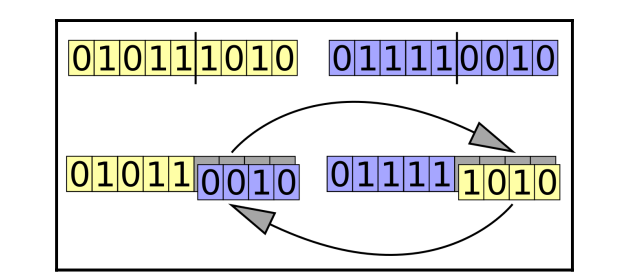
\includegraphics[width=0.5\textwidth]{cruza2puntos.png}
  \caption{Cruza de dos puntos}\label{fig:cr2puntos}
\end{figure}


\begin{lstlisting}[language=Python]
def cxTwoPoint(ind1, ind2):
    """Executes a two-point crossover on the input :term:`sequence`
    individuals. The two individuals are modified in place and both keep
    their original length.

    :param ind1: The first individual participating in the crossover.
    :param ind2: The second individual participating in the crossover.
    :returns: A tuple of two individuals.

    This function uses the :func:`~random.randint` function from the Python
    base :mod:`random` module.
    """
    size = min(len(ind1), len(ind2))
    cxpoint1 = random.randint(1, size)
    cxpoint2 = random.randint(1, size - 1)
    if cxpoint2 >= cxpoint1:
        cxpoint2 += 1
    else:  # Swap the two cx points
        cxpoint1, cxpoint2 = cxpoint2, cxpoint1

    ind1[cxpoint1:cxpoint2], ind2[cxpoint1:cxpoint2]
        = ind2[cxpoint1:cxpoint2], ind1[cxpoint1:cxpoint2]

    return ind1, ind2
\end{lstlisting}


El método de mutación seleccioand es mutShuffleIndexes (también podria se
mutFlipBit), en el cual se modifica el orden los números que componen al vector, dando lugar a por ejemplo:

(figura con ejemplo)
